\chapter{Introduction}
\label{chap:introduction}

\noindent
	Analysing patterns of morphological diversity has important implications for our understanding of ecological and evolutionary traits. For example, from a functional ecology perspective, morphological characteristics of limbs inform us about locomotory style \citep[e.g.][]{Bou1987} and the trophic niches associated with particular dental morphologies affect speciation and diversification rates through time \citep{Price2012}. Morphological diversity is also an important aspect of evolutionary patterns such as adaptive radiations and convergent evolution. High morphological diversity is a unifying \citep{Losos2010a, Olson2009}, although not defining \citep{Glor2010, Olson2009}, characteristic of adaptive radiations. Furthermore, analysing morphological convergences in groups such as freshwater cichlid fish \citep{Muschick2012} and anole lizards \citep{Mahler2013} gives interesting insights into the relative repeatability of evolution \citep{Losos2011}.
% NC: It's anole lizards or \textit{Anolis} lizards

%Need quantitative: combined the two paragraphs together
	Although studies of morphological diversity have clear implications for our understanding of ecological and evolutionary patterns, apart from a few examples \citep[e.g.][]{Ruta2013, Goswami2011, Brusatte2008}, it is still common to study morphological diversity from a qualitative rather than quantitative perspective. However, we need to quantify the morphological similarities and differences among species to gain a better understanding of their ecological interactions and evolutionary history. Unfortunately, morphological diversity is difficult to quantify. Studies are inevitably constrained to measure the diversity of specific traits rather than overall morphologies \citep{Roy1997}. In addition, our perception of morphological diversity is influenced by the trait being used. One study of pterosaurs demonstrated that comparing the diversity of different morphological traits using varying methods produced similar results \citep{Foth2012}. However, it remains unclear whether this finding can be applied to all vertebrate groups: in some species, comparing the relative diversity of cranial and limb morphologies may yield different results \citep{Foth2012}. Furthermore, linear measurements of morphological traits can restrict our understanding of overall morphological variation:  morphometric studies based on caliper measurements of particular features often fail to capture the overall shape of a specific structure \citep{Slice2007}. A distance matrix of measurements between specific points is unlikely to give a completely accurate representation of a three dimensional structure \citep{Rohlf1993}.
	
	Comparing shape variation using single, linear measurements may be appropriate in some cases \citep[e.g.][]{Morales2013} but the issues highlighted above are important limitations to consider. Geometric morphometric approaches help to overcome some of the issues associated with traditional morphological studies by using a system of Cartesian landmark coordinates to define anatomical points \citep{Adams2004}. 
	
	Geometric morphometric techniques capture more of the true, overall anatomical shape of particular structures \citep{Mitteroecker2009}. There are two main approaches to geometric morphometrics: two dimensional (2D) and three dimensional studies (3D). Three dimensional studies use 3D-scanners to create complete, virtual representations of anatomical features. However, the cost and time involved in scanning objects makes this approach impractical for large, cross-taxa comparisons of shape variation. In contrast, 2D geometric morphometric studies are commonly used to analyse three-dimensional morphological shape and are appropriate for cross-species comparisons \citep[e.g.][]{Muschick2012, Panchetti2008, Wroe2007, Marcus2000}  
		
	Of course there are potential biases associated with 2D morphometric approaches as they rely on 2D landmarks to represent 3D anatomical features. However, sensitivity analyses have demonstrated that bias from 2D representation of 3D structures is unlikely to be a significant issue for interspecific studies as the overall shape variation among species is greater than discrepancies introduced by using 2D morphometric techniques \citep{Cardini2014}. In addition, using multiple 2D approaches to analyse 3D shape (e.g. comparing skull shape using dorsal, ventral and lateral views) generates more robust shape variation results instead of summarising 3D anatomical shape using just one set of 2D photographs \citep{Arnqvist1998}.
	

	
	In this thesis, I apply 2D geometric morphometric techniques to quantify morphological diversity in a Family of small mammals, the tenrecs. Tenrecs (Afrosoricida, Tenrecidae) are a morphologically diverse group that is commonly cited as an example of both convergent evolution and an adaptive radiation \citep{Soarimalala2011, Eisenberg1969}. The Family is comprised of 34 species, 31 of which are endemic to Madagascar \citep{Olson2013}. Body masses of tenrecs span three orders of magnitude (2.5 to > 2,000g); a greater range than all other Families, and most Orders, of living mammals \citep{Olson2003}. Within this vast size range there are tenrecs which convergently resemble shrews (\textit{Microgale} tenrecs), moles (\textit{Oryzorictes} tenrecs) and hedgehogs \citep[\textit{Echinops} and \textit{Setifer} tenrecs,][Figure \ref{fig:tenrecs}]{Eisenberg1969}. Their similarities include examples of morphological, behavioural and ecological convergence \citep{Soarimalala2011}. Tenrecs are one of only four endemic mammalian clades in Madagascar and the small mammal species they resemble are absent from the island \citep{Garbutt1999}. Therefore, it appears that tenrecs represent an adaptive radiation of species which filled otherwise vacant ecological niches and, in doing so, developed convergent similarities with other small mammal species \citep{Soarimalala2011}.
	
	The similarities among tenrecs and other small mammals are even more remarkable when you consider their phylogenetic history. Tenrecs were originally classified within the general "Insectivora" clade and only molecular studies revealed their true phylogenetic affinities within the Afrotherian mammals \citep{Stanhope1998}. Therefore, despite initial appearances, tenrecs are more closely related to elephants, manatees and aardvarks than they are to shrews, moles or hedgehogs. 
%--------------------------------------------------
%SF I added attribution for each image
\begin{figure}[h] 
  \centering
  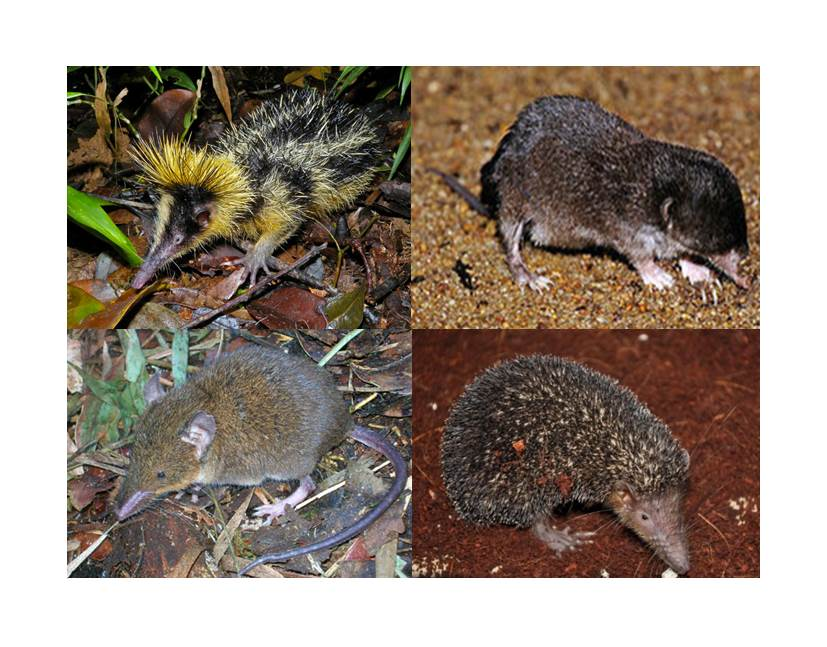
\includegraphics[width=14cm, height=14cm, keepaspectratio=true]{Introduction/FourTenrecs.jpg}
    \caption[Examples of tenrec species]
    {Examples of the morphological variety in the tenrec Family. Clockwise from top left: lowland streaked tenrec (\textit{Hemicentetes semispinosus}, \copyright Frank Vassen), mole-like rice tenrec (\textit{Oryzorictes hova}, \copyright Karl Lehmann), Talazac's shrew tenrec (\textit{Microgale talazaci}, \copyright Voahangy Soarimalala) and a greater hedgehog tenrec (\textit{Setifer setosus}, \copyright Lubom\'{i}r Kl\'{a}til).}
  \label{fig:tenrecs}
  \end{figure}
  
%Links to image sources: H semi http://goo.gl/epDL97, O. hov http://goo.gl/Uta02h, microgale http://goo.gl/o1ODXA, setifer http://www.biolib.cz/en/image/id160938/
%--------------------------------------------------
%Need a quantitative approach to test these ideas
	Although tenrecs are often cited as an example of both an adaptive radiation and exceptional convergent evolution, these claims have not been investigated quantitatively. There are qualitative similarities among the hind limb morphologies of tenrecs and several other unrelated species with similar locomotory styles \citep{Salton2009} but the degree of morphological similarity has not been established. Adaptive radiations and convergent evolution are separate evolutionary processes yet morphological diversity is common to both: morphological diversity is an important \citep[though not defining,][]{Olson2009} feature of adaptive radiations \citep{Losos2010a} and it also informs our understanding of convergent phenotypes \citep{Muschick2012}. Therefore, it is important to quantify patterns of morphological diversity in tenrecs to gain an insight into their evolution. My thesis is the first study to address this issue. 

%---------------------------------------------------


	Here I present the first quantitative study of patterns of morphological diversity in tenrecs. I compiled an extensive data set of morphological characteristics in tenrecs, their closest relatives (golden moles; Afrosoricida, Chrysochloridae) and the mammals that they convergently resemble. Chapter \ref{chap:methods} includes details about my data collection and the general morphometrics analyses which form the basis for my study. I collected morphological data on the skulls, limbs and skins from 366 specimens representing 99 species of small mammals. I used a subset of these data in Chapter \ref{chap:disparity} to quantify the morphological diversity of tenrec skulls compared to their closest relatives, the golden moles. Details of the remaining data can be found in Appendix \ref{appendix}: these data represent a significant resource for future studies. Finally, in Chapter \ref{chap:discussion}, I discuss the implications of my findings within the context of our understanding of tenrec evolution. My results reveal new insights into our understanding of morphological variety in tenrecs and prompt many new questions and possible avenues for further research.


